\begin{figure}[H]
\centering
\shorthandoff{<>}
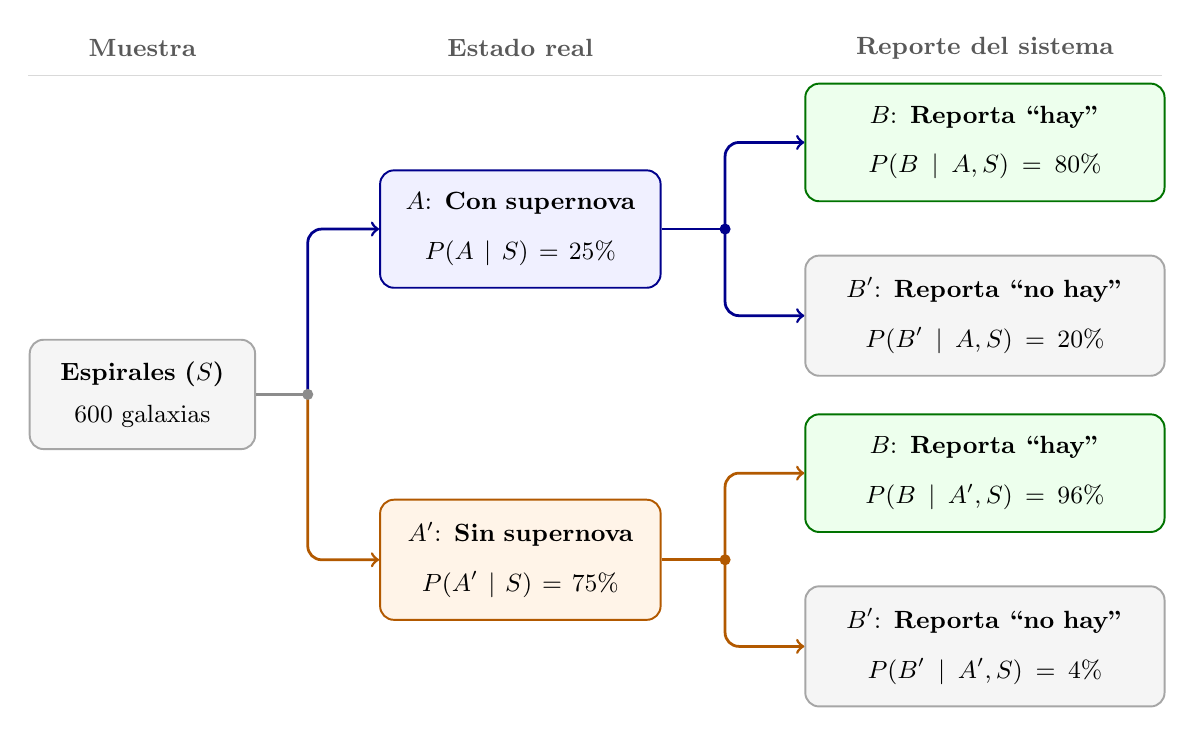
\begin{tikzpicture}[
  font=\small,
  eventbox/.style={rounded corners=5pt,align=center,minimum height=1.2cm,inner sep=8pt,line width=0.7pt},
  statebox/.style={eventbox,text width=3cm},
  reportbox/.style={eventbox,text width=4cm},
  connection/.style={->,line width=1pt,rounded corners=5pt},
  heading/.style={font=\small\bfseries,text=black!65,align=center}
]
  \node[heading] at (0,4.4) {Muestra};
  \node[heading] at (4.8,4.4) {Estado real};
  \node[heading] at (10.7,4.4) {Reporte del sistema};
  \draw[black!15] (-1.45,4.05) -- (12.95,4.05);

  \node[eventbox,draw=black!35,fill=black!4,text width=2.3cm] (spiral) at (0,0)
    {\textbf{Espirales ($S$)}\\[4pt]600 galaxias};

  \node[statebox,draw=blue!55!black,fill=blue!6] (supernova) at (4.8,2.1)
    {$A$: \textbf{Con supernova}\\[7pt]
    $P(A\mid S)=\boldsymbol{25\%}$};
  \node[statebox,draw=orange!70!black,fill=orange!9] (nosupernova) at (4.8,-2.1)
    {$A'$: \textbf{Sin supernova}\\[7pt]
    $P(A'\mid S)=\boldsymbol{75\%}$};

  \node[reportbox,draw=green!45!black,fill=green!7] (detected) at (10.7,3.2)
    {$B$: \textbf{Reporta ``hay''}\\[7pt]
    $P(B\mid A,S)=\boldsymbol{80\%}$};
  \node[reportbox,draw=black!35,fill=black!4] (missed) at (10.7,1)
    {$B'$: \textbf{Reporta ``no hay''}\\[7pt]
    $P(B'\mid A,S)=\boldsymbol{20\%}$};
  \node[reportbox,draw=green!45!black,fill=green!7] (reported) at (10.7,-1)
    {$B$: \textbf{Reporta ``hay''}\\[7pt]
    $P(B\mid A',S)=\boldsymbol{96\%}$};
  \node[reportbox,draw=black!35,fill=black!4] (absent) at (10.7,-3.2)
    {$B'$: \textbf{Reporta ``no hay''}\\[7pt]
    $P(B'\mid A',S)=\boldsymbol{4\%}$};

  \draw[line width=1pt,black!45] (spiral.east) -- (2.1,0);
  \draw[connection,blue!55!black] (2.1,0) -- (2.1,2.1) -- (supernova.west);
  \draw[connection,orange!70!black] (2.1,0) -- (2.1,-2.1) -- (nosupernova.west);
  \fill[black!45] (2.1,0) circle (2pt);

  \draw[line width=1pt,blue!55!black] (supernova.east) -- (7.4,2.1);
  \draw[connection,blue!55!black] (7.4,2.1) -- (7.4,3.2) -- (detected.west);
  \draw[connection,blue!55!black] (7.4,2.1) -- (7.4,1) -- (missed.west);
  \fill[blue!55!black] (7.4,2.1) circle (2pt);

  \draw[line width=1pt,orange!70!black] (nosupernova.east) -- (7.4,-2.1);
  \draw[connection,orange!70!black] (7.4,-2.1) -- (7.4,-1) -- (reported.west);
  \draw[connection,orange!70!black] (7.4,-2.1) -- (7.4,-3.2) -- (absent.west);
  \fill[orange!70!black] (7.4,-2.1) circle (2pt);
\end{tikzpicture}
\shorthandon{<>}
\caption{Árbol de probabilidades para las galaxias espirales. $A$ y $A'$ representan la presencia y ausencia real de supernova; $B$ y $B'$, los reportes del sistema. La probabilidad de cada recorrido desde un nodo al siguiente se muestra en el recuadro de destino. Todas están condicionadas a $S$. Los complementos añadidos son $75\%=100\%-25\%$, $20\%=100\%-80\%$ y $96\%=100\%-4\%$.}
\label{fig:arbol-espirales}
\end{figure}
